\chapter{Problem Analysis}\label{ch:problem}
This chapter entails an analysis of the problem, which is the research question's foundation.
It is crucial, as the quality of requirements ultimately determines the quality of the
subsequent analysis.

Requirements for a software system that involves \ac{ML} and thus \ac{DL} differs from
the traditional approach. The data-driven software components are not entirely defined by the
programmer but are influenced by data.
The system acts with dependency on the test data~\citep{siebert_construction_2021}.
This poses a challenge in determining requirements and measuring the quality of
results~\citep{nakamichi_requirements-driven_2020}.
Instead of categorizing functional and non-functional requirements, like for traditional
software projects~\citep{zowghi_requirements_2014}, qualities that a \ac{MLS} must possess
are defined.

\section{Use Case}
A use case can depict the problem.
This use case sets the foundation for determining requirements for an
approach because qualities derive from the intended purpose of
use~\citep{siebert_construction_2021}.
Table~\ref{tb:useCaseQualities} gives an overview of the relevant properties derived
from the use case.
\begin{table}[ht]
    \centering\scriptsize
    \begin{tabular}{c l}
        \textbf{Offline Capabilities} & Perform extraction process offline \\
        \textbf{Alphanumeric recognition}    & Recognize alphanumeric strings such as serial \\
                                    & numbers \\
        \textbf{Semantics retention} & Retain semantics given implicitly be space, \\
                            & strucure and rotation of text in labels \\
    \end{tabular}
    \caption{Qualities specific to use case --- exclusion criterias\label{tb:useCaseQualities}}
\end{table}
For this thesis, the primary use case is as follows:
A technician takes a photo of a device label with his smartphone.
For this, the technician is situated in locations like a cable shaft.
Due to this, there is no internet availability.
The process from taking the image to storing the extracted text must work offline safely.
The resulting image contains printed textual information, which an application on the smartphone must
extract.

The space and structure of this information can vary from label to label (see
Figure~\ref{fig:examples}).
The text does not have to be oriented horizontally.
The text, spacing, and structure carry semantic information, which can be crucial for later
processing in the scope of a business process~\citep{chen_text_2021}.
The goal is to extract the text and preserve semantics that is implicitly provided through
structure and space.
This means text and the respective coordinates, height, width, and a possible rotation angle must
be output as a result~\citep{yang_learning_2021}.
Those values can then be transformed into other formats such as JSON or HTML as needed.
\begin{figure}[h]
    \centering
    \subfigure[Positive example\label{fig:good-example}]{\includegraphics[width=0.40\textwidth]
        {img/Image-Example-Positive.jpg}}
    \subfigure[Negative example\label{fig:bad-example}]{\includegraphics[width=0.40\textwidth]
        {img/Image-Example-Negative.jpg}}
    \caption{Examples for label images\label{fig:examples}}
\end{figure}
% XXX: use concept of representation for semantics retention

In addition to this, the labels can contain arbitrary alphanumeric strings such as serial numbers
(see figure~\ref{fig:examples}).
This results in the requirement that the \ac{DL} model recognizes sequences that
are not part of a predefined lexicon~\citep{ghosh_visual_2017,chen_text_2021}.
The qualities for the \ac{MLS} that can be derived directly from the use case (see
Table~\ref{tb:useCaseQualities}) can be regarded as excluding criteria because an approach
that does not possess the qualities in question cannot be regarded as viable for the use case.

\section{Quality Identification}
In the article~\cite{ashmore_assuring_2021}, the qualities are identified and assigned to different
challenges in working with \ac{MLS}: Development, production,
organizational challenges.
Because only the Model Selection substage of the lifecycle is performed, the defined challenges and
their qualities are not relevant for this thesis, as they concern the operational aspect of
\acp{MLS}.

In~\cite{nakamichi_requirements-driven_2020,siebert_construction_2021}, systematic
identification and documentation of qualities are detailed.
In \acp{MLS} various entities interact to produce the desired functionality.
The paper~\cite{nakamichi_requirements-driven_2020} suggests that to evaluate
the qualities adequately, it is essential to consider the model and the entire \ac{MLS}
(see Figure~\ref{fig:MLS}).
\begin{figure}[ht]
    \centering
    {\scriptsize%
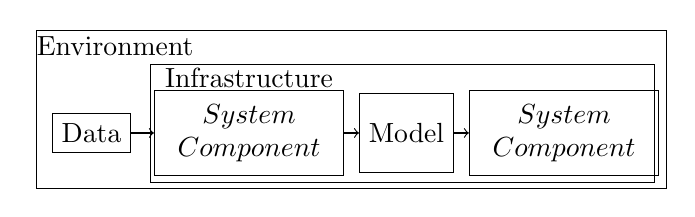
\begin{tikzpicture}
    \node (EnvBox) [rectangle,draw,minimum height =2cm, minimum width=8cm] at (0,0) {};
    \node (Env) at (-3, 0.8) {Environment};

    \node (InfrBox)[rectangle,draw,minimum height =1.5cm, minimum width=6.4cm] at (0.65,-0.18) {};
    \node (Infr) at (-1.3, 0.4) {Infrastructure};

    \node (Data) [rectangle,draw,minimum height =0.5cm, minimum width=0.5cm] at (-3.3,-0.3) {Data};
    \node (Sys1) [rectangle,draw,minimum height =1cm, minimum width=1cm] at (-1.3,-0.3)
        {$\begin{array}{c} \text{System} \\ \text{Component} \end{array}$};
    \node (Model)[rectangle,draw,minimum height =1cm, minimum width=1cm] at (0.7,-0.3) {Model};
    \node (Sys2) [rectangle,draw,minimum height =1cm, minimum width=1cm] at (2.7,-0.3)
        {$\begin{array}{c} \text{System} \\ \text{Component} \end{array}$};

    \draw [->] (Data) -- (Sys1);
    \draw [->] (Sys1) -- (Model);
    \draw [->] (Model) -- (Sys2);

\end{tikzpicture}
}

    \caption[Machine learning system entities]{%
        Machine learning system entities~\citep{nakamichi_requirements-driven_2020}\label{fig:MLS}
    }
\end{figure}
These entities are data, model, environment,
system/infrastructure~\citep{nakamichi_requirements-driven_2020, siebert_construction_2021}.
The article~\cite{siebert_construction_2021} differentiates between system and infrastructure.

The infrastructure represents given hardware and available libraries, whereas the system depicts
the software that surrounds the model in the runtime environment.
The data view pertains to development and runtime data~\citep{siebert_construction_2021}.
The model consists of subcomponents organized in a directed acyclic graph building a
pipeline.
This directed acyclic graph depicts everything from processing the images to the extracted
information~\citep{siebert_construction_2021}.
The environment entity covers the external aspects of the \ac{MLS}, which may interact with
it~\citep{siebert_construction_2021}.
In the scope of this work, the environment entails mainly the conditions in which images are taken.

For this thesis, the entities data and system cannot be regarded as given.
The entities environment and infrastructure are only loosely defined through the use case.
That is why the systematic approaches cannot be performed in the scope of this thesis.
For example,~\cite{siebert_construction_2021} propose to follow the systematic CRISP-DM approach of
identifying qualities.
It cannot be performed due to the lack of data and the other entities derived from the use case.

Table~\ref{tb:LiteratureQualitiesModel} lists all qualities that pertain to the model entity
and that were found in literature.
Different qualities are \textit{grouped} for their similarities.
Because of their properties, they can be evaluated jointly.
When documenting the identified qualities,
both~\cite{nakamichi_requirements-driven_2020} and~\cite{siebert_construction_2021} define a
meta-model for qualities that combines qualities with
measurement methods and values and assigns them to an entity of the \ac{MLS}.
The implementation and testing phases are not performed in the scope of this thesis, and the
difficulty in assessing the performance ahead of those phases prevents the evaluation
of measurements.

Additionally, experimental results from literature can only be compared as long as factors such as
hardware, platform, source code, configuration and dataset are uniform~\citep{arpteg_software_2018}.
Comparing models through the results of different papers is troublesome because different papers
might use different evaluation and testing environments~\citep{baek_what_2019}.
This applies to studies that present an overview, such as~\cite{chen_text_2021,long_scene_2021}.
These studies can only be regarded as guiding values because the performance for a specific dataset
cannot be predicted without testing on it~\citep{arpteg_software_2018}.
That is why targets for measurements are not defined, as evaluation would only deliver a false
sense of certainty.

\begin{table}[h]
    \centering\scriptsize
    \begin{tabular}{p{.4\textwidth} p{.6\textwidth}}
        \textbf{Quality} & \textbf{Sources} \\
        \toprule
        \textit{Appropriateness} \\
        Appropriateness &~\cite{siebert_construction_2021} \\
        Suitability &~\cite{siebert_construction_2021} \\
        Model Fitness --- Quality of Output Data &~\cite{nakamichi_requirements-driven_2020} \\
        \midrule
        \textit{Performance} \\
        Performance &~\cite{ashmore_assuring_2021,vogelsang_requirements_2019} \\
        Accuracy &~\cite{nakamichi_requirements-driven_2020} \\
        Model Fitness --- Degree of Correctness &~\cite{nakamichi_requirements-driven_2020,
                                                    zhang_machine_2020} \\
        Development correctness &~\cite{siebert_construction_2021} \\
        Relevance / Bias-Variance tradeoff &~\cite{siebert_construction_2021, zhang_machine_2020} \\
        Trained Model Generalization Performance Appropriateness
                                                    &~\cite{nakamichi_requirements-driven_2020} \\
        \midrule
        \textit{Robustness} \\
        Robustness &~\cite{ashmore_assuring_2021, hu_towards_2020, siebert_construction_2021} \\
        Robustness Against Change of Input Data &~\cite{nakamichi_requirements-driven_2020} \\
        Robustness Against Noise Data &~\cite{nakamichi_requirements-driven_2020} \\
        \midrule
        \textit{Reusability} &~\cite{ashmore_assuring_2021} \\
        \midrule
        \textit{Interpretability} \\
        Interpretability &~\cite{ashmore_assuring_2021, siebert_construction_2021, zhang_machine_2020}\\
        Understandability &~\cite{nakamichi_requirements-driven_2020} \\
        Transparency &~\cite{arpteg_software_2018} \\
        Model Explainability &~\cite{vogelsang_requirements_2019} \\
        Comprehensibility &~\cite{ashmore_assuring_2021} \\
        Comprehensiveness &~\cite{ashmore_assuring_2021} \\
        \midrule
        \textit{Fairness}\\
        Fairness &~\cite{siebert_construction_2021, zhang_machine_2020} \\
        Freedom from Discrimination &~\cite{vogelsang_requirements_2019} \\
        \midrule
        \textit{Performance Efficiency} \\
        Resource Utilization &~\cite{siebert_construction_2021,
                                nakamichi_requirements-driven_2020} \\
        Execution efficiency &~\cite{siebert_construction_2021} \\
        Temporal Performance &~\cite{nakamichi_requirements-driven_2020} \\
        \bottomrule
    \end{tabular}
    \caption{MLS qualities identified for model entity\label{tb:LiteratureQualitiesModel}}
\end{table}
\FloatBarrier%

\section{Quality Relevancy}\label{se:relevant-qualities}
In addition to the qualities that arise directly from the use case, the literature reveals several
common qualities in regards to \ac{MLS} (see Table~\ref{tb:LiteratureQualitiesModel}), some of which
can be regarded as relevant and others do not hold any relevance for the specific use case (see
Table~\ref{tb:condensedQualities}).
The qualities are taken from the literature covering \ac{ML} in general to literature
covering \ac{STS}.
Only qualities that concern the model will be looked at, as the model is the focus of this thesis.
The qualities may, however, be influenced by other entities.

\begin{table}[h]
    \centering\scriptsize
    \begin{tabular}{l l}
        \textbf{Relevant}                & \textbf{Irrelevant} \\
        \toprule
        Appropriateness         & Fairness  \\
        Performance             & Interpretability \\
        Robustness              & Reusability \\
        Performance efficiency  & \\
    \end{tabular}
    \caption{Condensed qualities for model entity\label{tb:condensedQualities}}
\end{table}

% Appropriateness
The appropriateness quality refers to the ability to perform the type of task required by
the use case~\citep{siebert_construction_2021,nakamichi_requirements-driven_2020}.
For this thesis, this applies to \ac{STS} models.
Additionally, the properties derived from the use case (see
Table~\ref{tb:useCaseQualities}) can be grouped under this quality.
The offline capabilities are always given in the approaches outlined in Chapter~\ref{ch:research}.
Semantics retention is controlled by the text representation output of the \ac{STD} model (axis-aligned,
multi-oriented, or quadrilateral bounding box, text/non-text map).
Alphanumeric recognition is dependent on how well \ac{STR} performs without a lexicon.

% Performance
`An ML model is performant if it operates as expected according to a measure (or set of measures)
that captures relevant characteristics of the model output'~\citep{ashmore_assuring_2021}.
For the performance quality, a measure is chosen depending on the type of task to be
solved~\citep{siebert_construction_2021}.
The F-Score is an example a of metric used to compare different
models~\citep{chen_text_2021, long_scene_2021}.
Performance is usually measured with a test dataset that is independent of training and validating
a model to approximate the generalization performance~\citep{goodfellow_deep_2016,
nakamichi_requirements-driven_2020}.

% Robustness
The robustness of a model concerns environmental uncertainty~\citep{ashmore_assuring_2021}.
Due to the uncontrolled environment in the practical aspect of taking the images on-site
beneficial image properties can not be guaranteed~\citep{chen_text_2021}.
Robust text extraction can be influenced by factors such as complex backgrounds, text form
(text rotation, font variability, arrangement), image noise (lighting conditions, blur,
interference, and low resolution), and access (perspective, shape of
text)~\citep{oyedotun_deep_2015,ghosh_visual_2017,chen_text_2021}.
Therefore, these properties have to be accounted for when determining the viability of an approach.
Some of these factors do not change the expected prediction (noise), others do (text
form)\cite{hu_towards_2020}.
An example of poor image quality regarding \ac{STS} can be seen in figure~\ref{fig:bad-example}.
Note that the datasets introduced in Section~\ref{se:sts} include the challenging image properties,
as \ac{STS} is defined with robustness in mind.
For example,~\cite{karatzas_icdar_2013,karatzas_icdar_2015,chng_total-text_2017} define their
challenge with different image properties concerned with robustness.
Additionally, \ac{STS} is differentiated from \ac{OCR} by solving more difficult reading problems
for more complex images~\citep{long_scene_2021,hu_gtc_2020,chen_text_2021,baek_what_2019}.
Therefore, the difference in performance and robustness is negligable for \ac{STS}.

% Performance efficiency
Performance efficiency addresses time and resource utilization when the model is in use.
This does not involve the training phase but the execution or
prediction~\citep{siebert_construction_2021}.
The efficiency refers to low latency needs and minimizing resource needs such as memory
usage or power consumption~\citep{nakamichi_requirements-driven_2020, siebert_construction_2021,
sourvanos_challenges_2018}.
This quality is crucial for mobile devices in conjunction with
\ac{DNN}~\citep{sourvanos_challenges_2018, niu_26ms_2019}.
The infrastructure heavily influences performance
efficiency~\citep{nakamichi_requirements-driven_2020, siebert_construction_2021}.
Because the efficiency needs fall mainly on the model, it is categorized as such and thus deemed
relevant in the scope of this thesis.

% Fairness
The first quality often found in research not relevant for the use case is fairness.
A fair model is free from discrimination bias.
For \ac{ML}, this can be a big problem since discrimination can be influenced through
explicit programming in terms of the model and through implicit knowledge from the
data~\citep{vogelsang_requirements_2019}.
For the use case, however, no relevance is attached.
The model can either recognize the text or fail the task.

% Interpretability
The interpretability of a model helps to justify the output~\citep{ashmore_assuring_2021}.
The interpretability is twofold: explain what the model has learned, explain how a model given the
input comes to the output~\citep{vogelsang_requirements_2019}.
This can be challenging for two reasons.
\ac{ML} models can be complex in size and structure~\citep{ashmore_assuring_2021}.
Modular processing pipelines are continuously replaced with end-to-end
models facilitating the tradeoff between interpretability and
performance~\cite{arpteg_software_2018}.

% Reusability
Another quality for a \ac{ML} model refers to how well a model intended for one task can be reused
for another related task.
This can be beneficial because transfer learning can speed up the training, thus reducing training
costs~\citep{ashmore_assuring_2021}.
Reusability is not relevant in the scope of this work as it targets the training phase of the
\ac{ML} lifecycle.
The identified relevant qualities will be used in Section~\ref{se:analysis} to provide
properties to judge the merits of a possible solution.
